\begin{opin}{\guscolor}{Gustavo}


El objetivo que pretende Manuel es el de concienciarnos de la utilidad práctica que tiene el uso de las pizarras digitales en el aula a la hora de la enseñanza.

Manuel indica que las claves para que algo tenga éxito en educación son 3:

\begin{itemize}
\item[1.]Que sea muy fácil. 
\item[2.]Que sea adaptable. Valido para cualquier asignatura. 
\item[3.]Que sea útil pedagógicamente. 
\end{itemize}

\subsubsection{Hoy Soy Feliz Porque Tengo Ayuda}

\textbf{H}oy \textbf{S}oy \textbf{F}eliz porque tengo \textbf{A}yuda.

El camino para conseguir ese éxito tiene que ver con el título del apartado.

\paragraph{H de Hardware}
Son las herramientas. Pero el importante es el que transmite que es EL PROFESOR. Tipos de hardware:

\begin{itemize}
\item Pizarra Digital Interactiva (PDI) 

\item Pizarra Digital Interactiva Portátil (PDiP). La que usa el profesor en su clase. Se puede usar desde cualquier lugar. Más económica, más flexible y con mayores posibilidades. 

\item Articlick. EVCD: Evaluacion continua Digital. 

\item Cámaras de documentos. Es barata y permite ver documentos y hacer anotaciones sobre ellos. 

\item Micrófonos y altavoces. 
\end{itemize}

\paragraph{S de Software}
Hay muchos tipos de software.

Las características del software asociado a la pizarra que nos mostró el profesor incluía:

\begin{itemize}
\item Una barra de herramientas personalizable y flotante sobre cualquier aplicación.  

\item Se permiten hacer anotaciones. Todas las anotaciones se guardan automáticamente.  

\item Se puede borrar lo que se quiera.  

\item Se pueden exportar a cualquier formato.  

\item Se puede guardar un video con sonido de cualquier explicación previo a darle a guardar. 

\item El lápiz hace de ratón: 
\begin{itemize}

\item Boton izquierdo: Punta 

\item Doble click: Botón central 

\item Botón derecho: último botón. 
\end{itemize}
\end{itemize}

Una vez explicadas las capacidades de la pizarra, Manuel nos mostró una serie de ejemplos de aplicación de simulaciones de mucha utilidad entre las que destacaría la “Graphing  calculator 3D” por encima de todas las demás ya que siempre cuesta mucho explicar cómo se representan los planos en el espacio y esta herramienta es absolutamente fantástica. Otras aplicaciones que también me resultaron interesantes fueron:
\begin{itemize}
\item[1.]La aplicación que te permite hacer simulaciones de caída de objetos y un péndulo. 

\item[2.]RM Easiteach con la que explica el movimiento de la tierra con respecto al sol y de la luna con respecto a la tierra. 

\item[3.]Otra aplicación explica los colores primarios y su mezcla que produce los colores complementarios que son los de la impresora 
\end{itemize}

\paragraph{F de Formación}
El profesor tiene que tener un curso presencial motivador

Tiene que existir un curso online

\paragraph{A de Ayuda}
Tienen que existir tanto el apoyo como las ayudas al profesor. IMC

\index{EVCD}\textbf{EVCD}: Evaluacion continua Digital
Por último, hicimos una demostración en clase pasa a explicar la evaluación continua con el programa VPAD. Encontré esta aplicación superútil dado que se pueden hacer evaluaciones interactivas de mucha utilidad.

Además añadiría que no hace falta descargarsela desde el móvil ya que se puede utilizar desde cualquier cliente web.

Hay otros programas como Flow, Plickers y Kahoot en internet en los que también se pueden hacer evaluaciones interactivas.

\paragraph{Street View y realidad virtual de una casa}
Con Manuel también aprendí que con el Street View de Google se puede hacer una foto de una habitación de casa y luego verla con unas gafas de realidad virtual o directamente con un móvil con visión de 360º. Sencillamente impresionante


\end{opin}

\begin{opin}{\victorcolor}{Víctor}

Hoy hemos visto utilizar una \index{PDi(P)}\textbf{PDi(P)}\textbf{ - Pizarra Digital interactiva (Portátil)} y unas cuantas aplicaciones muy útiles para trabajar con tics en el aula.

Entre ellas: Graphing calculator 3D (para dibujar superficies e intersecciones de superficies).
%
Esta herramienta complementa muy bien a geogebra, puesto que los problemas de geometría de segundo de bachillerato son en tres dimensiones y geogebra no tiene opción a dibujar en 3 dimensiones.

Otra herramienta simulaba el comportamiento de objetos atraídos por la fuerza de la gravedad. 
%
Lo primero es dibujar los objetos sin gravedad. Después, al activar la gravedad los objetos se mueven y se puede ver el comportamiento de un péndulo, de un lanzamiento vertical y estudiar a qué altura llega... ¡Los enunciados de los problemas pueden ser vídeos!

A la hora de dibujar en matemáticas, estas herramientas son geniales. Ayudan a visualizar mucho mejor y sobretodo, ahorran mucho tiempo de hacer los dibujos.

La explicación sobre los colores primarios de 15 segundos es la mejor explicación que he escuchado en la vida. 
%
Tener el \textit{flash} sobre los colores primarios de la luz permite mezclaros en el momento y moverlos sin apenas esfuerzo. 
%
Al mezclarlos, se comprueba claramente que son los colores complementarios (los colores que utilizan las impresoras para conseguir todos los demás).

Ha sido muy constructiva esta sesión, aunque hubiera estado mejor poder probarlas, ya que escribir sin mirar a dónde estás escribiendo no me parece algo muy intuitivo. 
%
¿Cuánto entrenamiento hace falta para acostumbrarse?
%
¿Cómo es la curva de aprendizaje?


\end{opin}

\begin{opin}{\pedrocolor}{Pedro}


Esta sesión ha resultado realmente enriquecedora. Ha sido mi primera aproximación a las pizarras digitales gracias a Manuel García. Su gran capacidad de síntesis me permitió tener una visión general de los cuatro campos que cubren las pizarras digitales: Hardware, Software, Formación y Ayuda.

\begin{itemize}

\item \textbf{Hardware:}
\begin{itemize}

\item \textbf{PDIP} (Pizarra Digital Interactiva Portátil). Nos ha mostrado la facilidad de utilización en el aula. Permite poder impartir clase desde cualquier sitio de la sala, cedérsela a los alumnos, y con posibilidad de conectar entre si hasta 9,  simultáneamente repartidas por la clase. 

\begin{minipage}[hbtp]{1.0\linewidth}
\centering
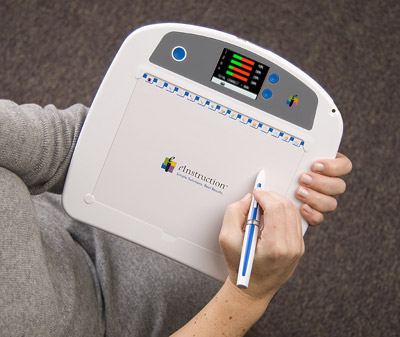
\includegraphics[scale=0.4]{img/pdipedro.jpg}
\captionof{figure}{Pizarra Digital Interactiva Portátil}
\end{minipage}

 
\item \textbf{PDI} (Pizarra Digital Interactiva) pese a no tener una disponible en el aula, nos ha explicado que los recursos que aporta una buena utilización de la misma son infinitos. 

\item Equipo Visualizador Cámara de Documentos nace como una evolución del proyector de diapositivas. Permite digitalizar cualquier material y compartirlo en clase. En algunos casos, permiten hasta realidad aumentada con presentaciones 3D. 

\begin{minipage}[hbtp]{1.0\linewidth}
\centering
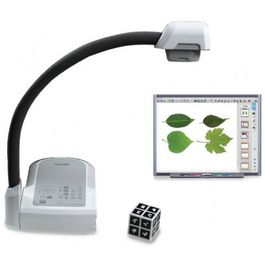
\includegraphics[scale=0.4]{img/pdipedro2.jpg}
\captionof{figure}{Equipo Visualizador Cámara de Documentos}
\end{minipage}
\end{itemize}
 
\item \textbf{Software:}
\begin{itemize}

\item \textbf{INTERWRITE Workspace} : Ofrece una gran cantidad de herramientas que permiten una mayor interactividad en el aula. Incluye reconocimiento de formas, herramientas de edición, etc. Considero que puede ser una herramienta bastante intuitiva. 

\begin{minipage}[hbtp]{1.0\linewidth}
\centering
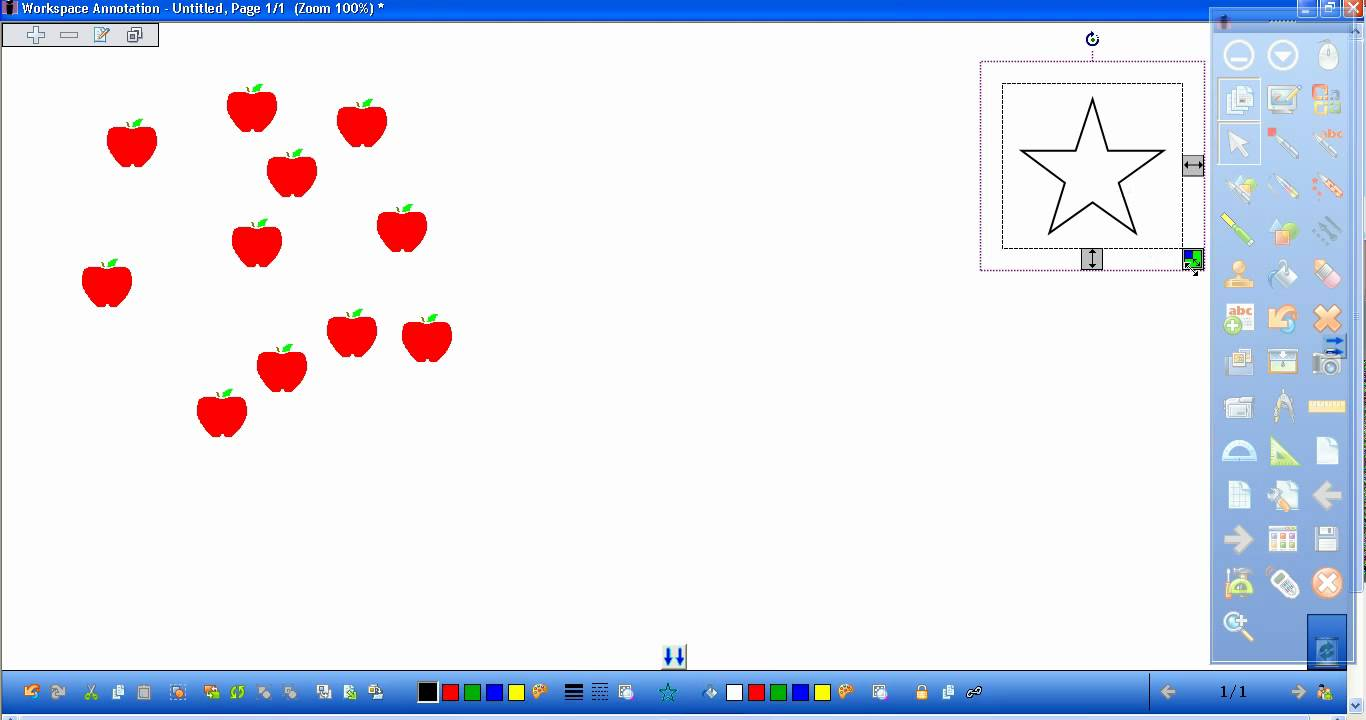
\includegraphics[scale=0.2]{img/pdipedro3.jpg}
%\captionof{figure}{...}
\end{minipage}

 
\item \textbf{Flow} : Permite realizar preguntas improvisadas en clase, y conseguir al instante un conocimiento exacto del nivel de compresión de cada alumno. 
Podemos también crear test y exámenes en cualquier formato (Word, Power-Point, Write, etc ). Dentro de la evaluación en el aula, cabe también destacar Plickers  y Kahoot.
        
\begin{minipage}[hbtp]{1.0\linewidth}
\centering
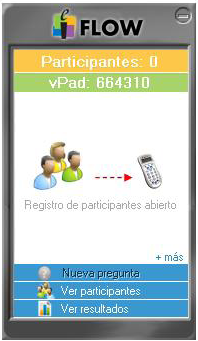
\includegraphics[scale=0.45]{img/pdipedro4.png}
%\captionof{figure}{...}
\end{minipage}

 
\item \textbf{Physics Illustrator} : Este software nos brinda la posibilidad de ver cómo la ley de la gravedad actúa sobre los objetos…un impacto, un desplazamiento, etc. 

 
\begin{minipage}[hbtp]{1.0\linewidth}
\centering
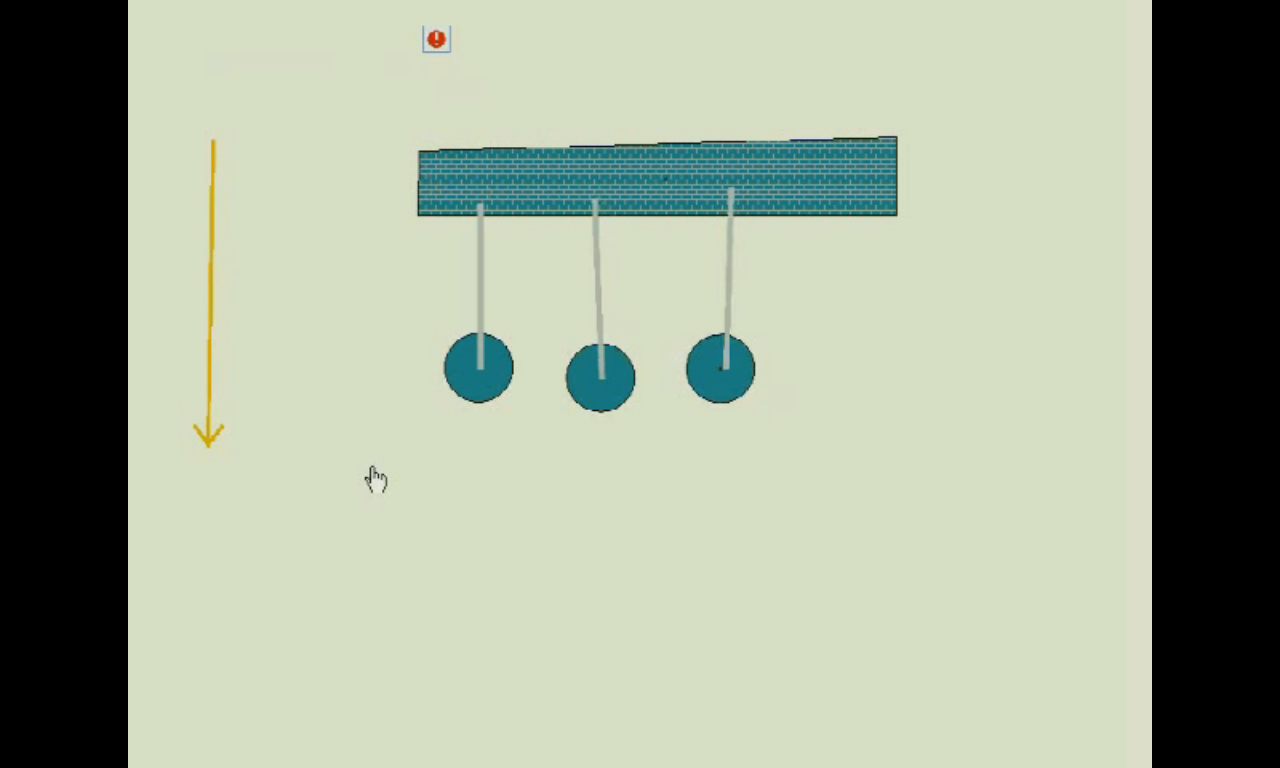
\includegraphics[scale=0.2]{img/pdipedro5.png}
%\captionof{figure}{...}
\end{minipage}

\item Existen otros tipos de software considerados como recursos a la hora de impartir clases, como:  \textbf{easiteach} y \textbf{Graphing Calculator}
 
\end{itemize}
\end{itemize}
\end{opin}

\begin{opin}{\virgicolor}{Virginia}
.


\end{opin}
